
%
% Gas Target NIM Paper 
%

%\documentclass[preprint,12pt]{elsarticle}

%% Use the option review to obtain double line spacing
%% \documentclass[authoryear,preprint,review,12pt]{elsarticle}

%% Use the options 1p,twocolumn; 3p; 3p,twocolumn; 5p; or 5p,twocolumn
%% for a journal layout:
%% \documentclass[final,1p,times]{elsarticle}
%\documentclass[final,1p,times,twocolumn]{elsarticle}
%% \documentclass[final,3p,times]{elsarticle}
%% \documentclass[final,3p,times,twocolumn]{elsarticle}
%% \documentclass[final,5p,times]{elsarticle}
\documentclass[final,5p,times,twocolumn]{elsarticle}

%% For including figures, graphicx.sty has been loaded in
%% elsarticle.cls. If you prefer /to use the old commands
\usepackage{amsmath, amssymb, amsfonts, latexsym}
\usepackage{epsfig}
\usepackage{subcaption}
\usepackage{adjustbox}
\usepackage{mathtools}
\usepackage{amssymb}
\usepackage{xcolor}
\usepackage{textcomp}
\usepackage{graphicx}

%% The amsthm package provides extended theorem environments
%% \usepackage{amsthm}

%% The lineno packages adds line numbers. Start line numbering with
%% \begin{linenumbers}, end it with \end{linenumbers}. Or switch it on
%% for the whole article with \linenumbers.
%% \usepackage{lineno}

\journal{Nuclear Instruments and Methods}

\begin{document}

\begin{frontmatter}

%% Title, authors and addresses

%% use the tnoteref command within \title for footnotes;
%% use the tnotetext command for theassociated footnote;
%% use the fnref command within \author or \address for footnotes;
%% use the fntext command for theassociated footnote;
%% use the corref command within \author for corresponding author footnotes;
%% use the cortext command for theassociated footnote;
%% use the ead command for the email address,
%% and the form \ead[url] for the home page:
%% \title{Title\tnoteref{label1}}
%% \tnotetext[label1]{}
%% \author{Name\corref{cor1}\fnref{label2}}
%% \ead{email address}
%% \ead[url]{home page}
%% \fntext[label2]{}
%% \cortext[cor1]{}
%% \address{Address\fnref{label3}}
%% \fntext[label3]{}

\title{Density Changes in Low Pressure Gas Targets}
%\title{Performance of the Hall A Tritium Target}

\author[Kent]{Sheren Alsalmi}
\author[UNH]{Nathaly Santiesteban}
\author[UNH]{Shujie Li}
\author[JLab]{David Meekins}

\address[Kent]{Kent State University}
\address[UNH]{University of New Hampshire}
\address[JLab]{Jefferson Lab}

\begin{abstract}

Hall A at Jefferson Lab has developed a new closed gas target system for the safe use of a tritium target. The system has been used in the 12 GeV era of experiments of the Continuous Electron Beam Accelerator Facility (CEBAF) using $^{3}H$, $^{3}He$, $^{2}H$, $^{1}H$ and $^{40}Ar$, at a maximum beam current of 
$22.5$ $\mu A$, during 2017 and 2018. The target cells were machined from solid  aluminum blocks and are all 25 cm long by 1.3 cm, with approximately 0.25 mm  windows for the beam entrance and exit. While the fill density is known, the  density of the gas when heated by the electron beam needs to be studied in 
order to calculate the correct cross sections from the experiments. As expected  from simulations, we find the density of the target dependent on the current of the electron beam going through the cell. A summary of the target system and the results of the study of the density change in each one of the targets will be summarized.

\end{abstract}

\begin{keyword}
Density
\sep target system
\sep $^{3}H$, $^{3}He$, $^{2}H$, $^{1}H$
\sep CEBAF.

%% keywords here, in the form: keyword \sep keyword

%% PACS codes here, in the form: \PACS code \sep code
%% MSC codes here, in the form: \MSC code \sep code
%% or \MSC[2008] code \sep code (2000 is the default)
\end{keyword}
\end{frontmatter}

%% \linenumbers

%% main text
\section{Introduction}
\label{}
%%%%%

\section{Target System}


The tritium target was developed in Hall A at Jefferson Lab for the experiments E12-10103 \cite{marathon}, E12-11-112 \cite{E12-11-112}, E12-13-012 \cite{E12-13-012} and E12-14-009 \cite{E12-14-009}. The target ladder is shown in Figure \ref{ladder}, which allows a total of five cells, where one cells was a dummy target for background measurements. The main experiment will cycle between the $^{3}H$, $^{2}H$, $^{1}H $, $^{3}He$ target cells for most of the beam time. A modular design was used for the target ladder in order to install the tritium cell after all the other targets were placed. Particularly, the tritium cell was the only cell that was not filled in Jefferson Lab, it was filled in the Savannah River site tritium Enterprises (SRTE), and it was shipped in a Type A container that was located in Hall A at all time in Jefferson Lab, with only qualified personal access. The cell only was out of the container while it was inside the scattering chamber.

\begin{figure}
\centering
  % Se pueden incluir figuras jpeg al compilar con PDFLatex
  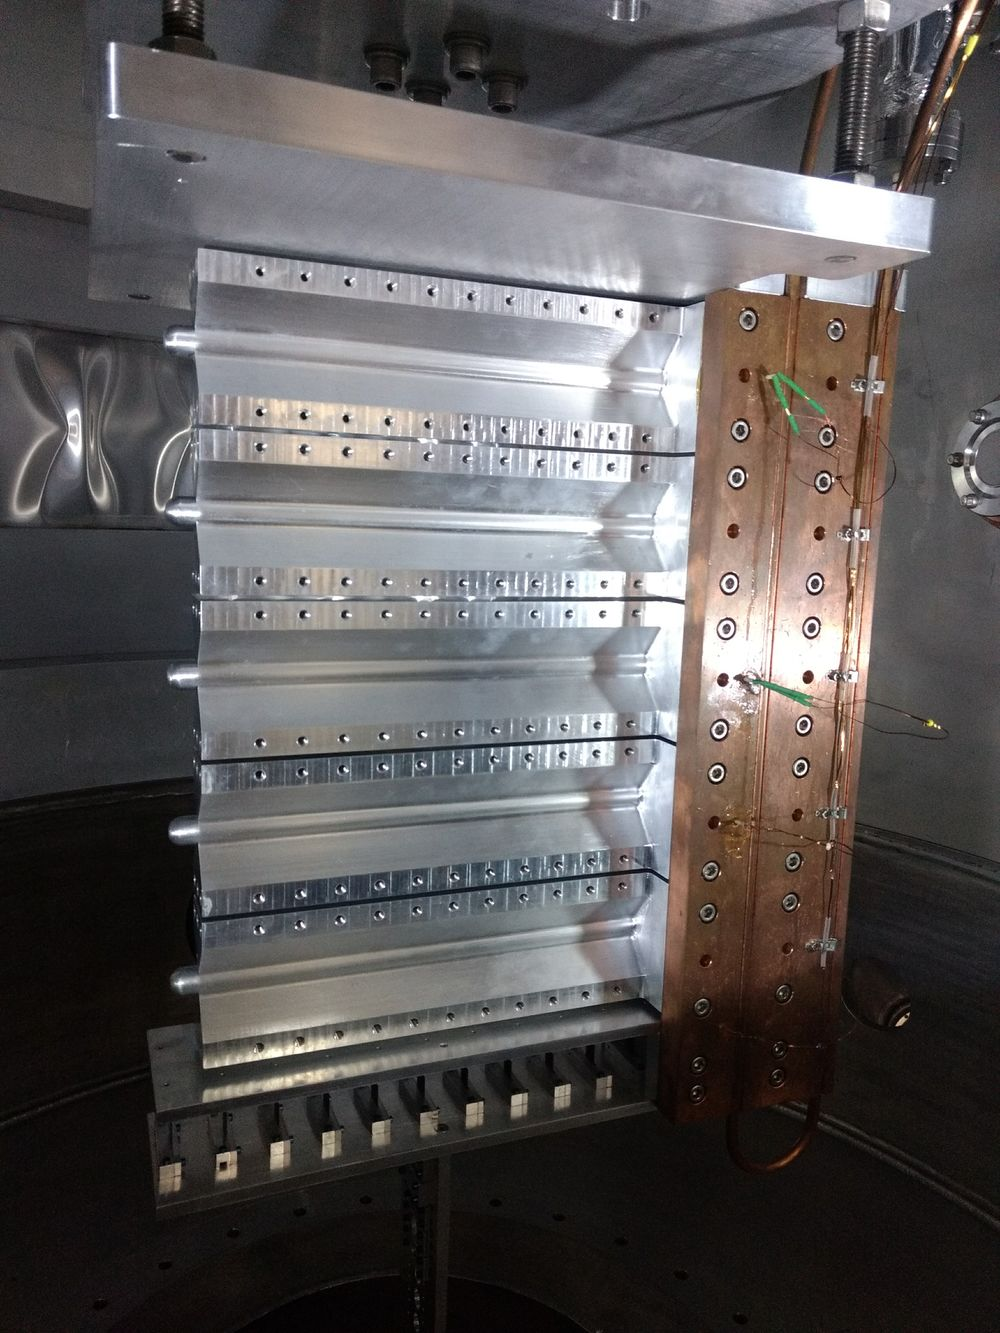
\includegraphics[width=6cm]{images/ladder.jpg}\\
  \caption{Ladder Assembly. Five cells were assembled during Fall 2017 to Spring 2018, $^{3}H$, $^{2}H$, $^{1}H $, $^{3}He$ and empty cell from top to bottom
 }\label{ladder}
\end{figure}

The vacuum system of the target provided containment/confinement during normal operations. This system includes the scattering chamber, the pumping system, the upstream beam isolation window and the dump line.  The scattering chamber has a volume of about 1900 liters and its configurations has been used in Hall A for more than 15 years. In this particular set of experiments, the chamber has an extra a beryllium (99.8$\%$) window to separate the upstream beamline and the scattering chamber, which also contains a collimator to minimize beam scraping on the target cell walls. The dump line was isolated from the scattering chamber using a gate valve during installation, maintenance and removal operations of the target cells. 

In addition, a special exhaust system was built to remove tritium from the scattering chamber and/or Hall A in a controlled manner in case the the tritium containment systems failed.  Furthermore, a temporary isolation room fixed to the scattering chamber, known as the transfer hut, was directly attached to the scattering chamber. The scattering chamber was connected directly to the exhaust system. Thus, the air pulled through the hut into the chamber went directly through the exhaust system.  

\subsection{Target Cell Characteristics}

The entire target assembly was cooled with $15K$ helium from the End Station Refrigerator (ESR). The $15K$ helium was preheated to $40K$ and used to cool a heat sink attached to the cell assemblies. This removed about $15W$ of heat that is generated by the electron beam. The beam current allowed on the tritium cell was limited to a maximum of $22$ $\mu A$ \cite{engreport}.


\begin{figure}
\centering
  % Se pueden incluir figuras jpeg al compilar con PDFLatex
  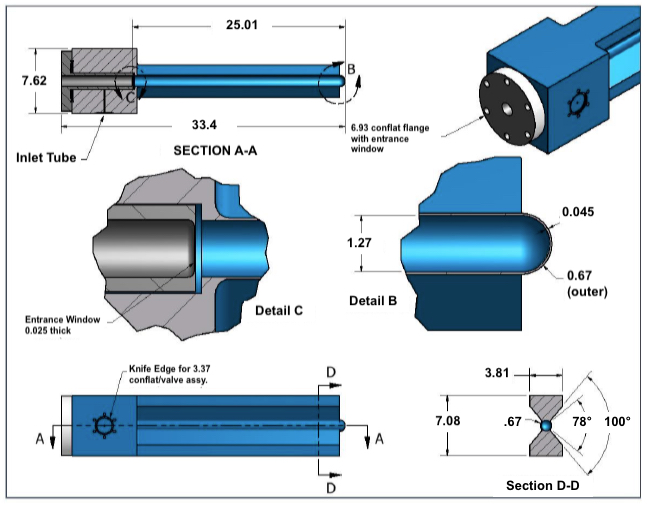
\includegraphics[width=11cm]{images/tritium_cell.jpg}\\
  \caption{Engineering design of an individual tritium gas target cell \cite{celldes}, using $cm$ units.
 }\label{cell}
\end{figure}

The gas targets are contained in a $25$ $cm$ long byt $1.27$ $cm$ diameter aluminum (7075-T6) sealed system, the target cell is shown in Figure \ref{}. The alloy 7075-T6 was chosen since it is tritium compatible, has high thermal conductivity, has high yield strength, and it is in routine use for target cells at JLab. The windows for beam entrance and exit would be $0.0254$ $cm$ and $0.0279$ $cm$ thick, respectively \cite{celldes}. 


The heat generated by the tritium decay is very small, about $50$ $mW$. The power deposited in the windows and gas is also relatively small with a beam current of $25$ $\mu A$. There will be a deposited power of approximately $4.7$ $W$ in the upstream window, $5.1$ $W$ in the downstream window, $3.8$ $W$ in the tritium gas, approximately $8.6$ $W$ in the hydrogen, deuterium and helium gases \cite{celldes}. 


\subsection{Target Cell Characteristics}

The target cell design was used in 5 gasses, in $Ar$ during February 2017, and $^{3}H$, $^{2}H$, $^{1}H $, $^{3}He$ during Fall 2017-Spring 2018. Each cell was measured along eight different points along the body according to Figure \ref{fig:cellconfig} and the measurements are summarized in Table \ref{tab:cell}. Furthermore, the filling parameters are summarized in the Table \ref{tab:fill_tar}, where the filling temperature was $291K$.

\begin{figure}
\centering
  % Se pueden incluir figuras jpeg al compilar con PDFLatex
  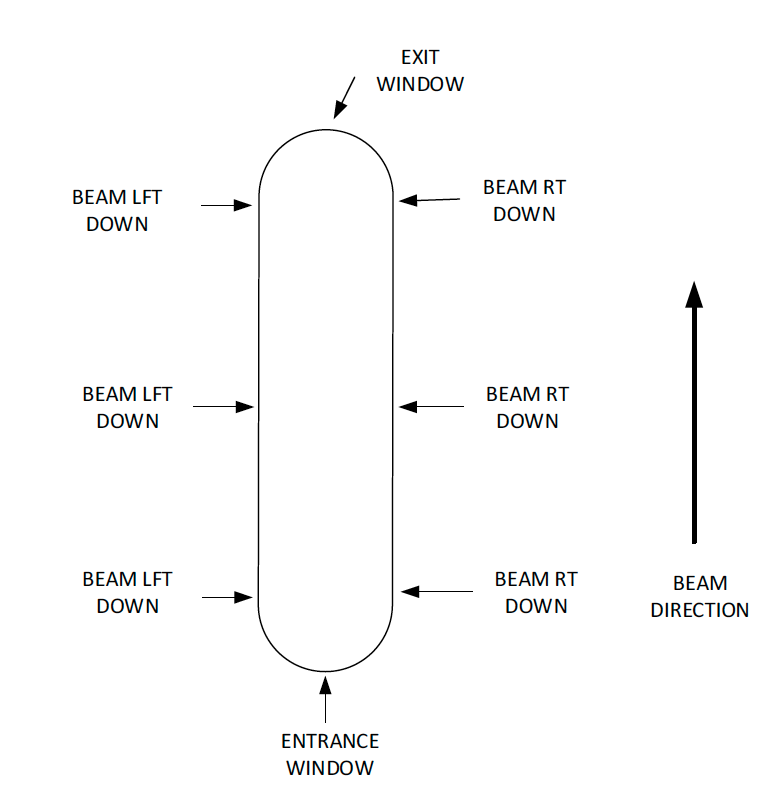
\includegraphics[width=8cm]{images/tgt_measurements.png}\\
  \caption{Measurement locations on the cells \cite{cellconfig}. 
 }\label{fig:cellconfig}
\end{figure}


\begin{table}[h!]
\centering
\begin{adjustbox}{width=1\textwidth}
\begin{tabular}{|c|c|c|c|c|c|c|}
\hline
Cell Position        & \begin{tabular}[c]{@{}c@{}} $Ar$ \\ Thickness $mm$\end{tabular}                & \begin{tabular}[c]{@{}c@{}}Empty Cell\\ Thickness $mm$\end{tabular} & \begin{tabular}[c]{@{}c@{}}$^{3}H$ Cell\\ Thickness $mm$\end{tabular} & \begin{tabular}[c]{@{}c@{}}$^{1}H$ Cell\\ Thickness $mm$\end{tabular} & \begin{tabular}[c]{@{}c@{}}$^{2}H$ Cell\\ Thickness $mm$\end{tabular} & \begin{tabular}[c]{@{}c@{}}$^{3}He$ Cell\\ Thickness $mm$\end{tabular} \\ \hline
Entrance               &        $0.254 \pm 0.0051$      & $0.254 \pm 0.0051$                                                  & $0.253 \pm 0.004$                                                     & $0.311 \pm 0.001$                                                     & $0.215 \pm 0.004$                                                     & $0.203 \pm 0.007$                                                      \\ \hline
Exit                    &     $0.279 \pm 0.0051$         & $0.279 \pm 0.0051$                                                  & $0.343 \pm 0.047$                                                     & $0.330 \pm 0.063$                                                     & $0.294 \pm 0.056$                                                     & $0.328 \pm 0.041$                                                      \\ \hline
Exit left              &       $0.4064 \pm 0.0051$       & $0.4064 \pm 0.0051$                                                 & $0.379 \pm 0.007$                                                     & $0.240 \pm 0.019$                                                     & $0.422 \pm 0.003$                                                     & $0.438 \pm 0.010$                                                      \\ \hline
Exit right              &      $0.4216 \pm 0.0051$                                                       & $0.4216 \pm 0.0051$                                                 & $0.406 \pm 0.004$                                                     & $0.519 \pm 0.009$                                                     & $0.361 \pm 0.013$                                                     & $0.385 \pm 0.016$                                                      \\ \hline
Mid left             &        $0.457 \pm 0.0051$                                                         & $0.457 \pm 0.0051$                                                  & $0.435 \pm 0.001$                                                     & $0.374 \pm 0.004$                                                     & $0.447 \pm 0.009$                                                     & $0.487 \pm 0.060$                                                      \\ \hline
Mid right             &       $0.432 \pm 0.0051$                                                         & $0.432 \pm 0.0051$                                                  & $0.447 \pm 0.004$                                                     & $0.503 \pm 0.005$                                                     & $0.371 \pm 0.012$                                                     & $0.478 \pm 0.007$                                                    \\ \hline
Entrance left      &         $0.508 \pm 0.0051$                                                          & $0.508 \pm 0.0051$                                                  & $0.473 \pm 0.003$                                                     & $0.456 \pm 0.010$                                                     & $0.442 \pm 0.005$                                                     & $0.504 \pm 0.003$                                                      \\ \hline
Entrance right     &		$0.424 \pm 0.0051$                            		 & $0.424 \pm 0.0051$                             & $0.425 \pm 0.003$                                & 
$0.457 \pm 0.006$                                & 
$0.332 \pm 0.011$                                & 
$0.477 \pm 0.011$                                 \\ \hline
\end{tabular}
\end{adjustbox}
\caption{Cell wall thickness measurements for all the gas targets. $Ar$ taken from \cite{ar_config} and for the other targets from \cite{cellconfig}.}
\label{tab:cell}
\end{table}

\begin{table}[h!]
\centering
\begin{tabular}{|c|c|c|c|}
\hline
Target   & Mass $(g)$           & \begin{tabular}[c]{@{}c@{}}$\rho t$\\ Target thickness\end{tabular} & \begin{tabular}[c]{@{}c@{}}Filling Pressure\\ ($psia$) \end{tabular} \\ \hline
$Ar$  & $1.943$              & $1.455 $ $g/cm^{2}$                                           & $500$  \\ \hline
$^{3}H$  & $0.102$              & $77 \pm 0.01$ $mg/cm^{2}$                                           & $203$                                                             \\ \hline
$^{3}He$ & $0.0713 $  & $53.4 \pm 0.6$ $mg/cm^{2}$                                         & $252.7$                                                           \\ \hline
$^{1}H$  & $0.094 $ & $70.8 \pm 0.4$ $mg/cm^{2}$                                         & $514.7$                                                           \\ \hline
$^{2}H$  & $0.1899 $ & $142.2 \pm 0.8$ $mg/cm^{2}$                                        & $514.7$                                                           \\ \hline
\end{tabular}
\caption{Gas target filling parameters at $291 K$. $Ar$ taken from \cite{ar_config} and for the other targets from \cite{cellconfig}. }
\label{tab:fill_tar}
\end{table}

\section{Experimental Hall A}

Hall A has $53$ $m$ of diameter and $17$ $m$ of height under a layer of concrete. Specifically, this data was taken in the Left High Resolution Spectrometer (LHRS). The basic components of the LHRS are three superconductingquadrupoles (Q) and one superconducting dipole (D) in a QQDQ configuration. The quadrupoles align the electron while the dipole determines the momentum of the electrons that get to the detector. After passing the magnets, the scattered electrons go through two Vertical Drift Chambers (VDCs), where the electrons ionize the gas inside the chambers, and with the information the position and angle of the trajectory are found. Then, the trigger scintillators s0 and s2, with the Cherenkov detector filled with CO2 between the trigger scintillator planes. They identify the electrons with $99 \%$  efficiency and has a threshold for pions of $4.8$ $GeV$ . Finally, the preshower and shower lead glasses blocks induce a cascade of pair production and bremsstrahlung radiation from energetic particles, which are used for the measurement of the energy of the electrons.


\section{Beam Current Monitor (BCM)}

The Beam Current Monitor (BCM) is the highest source of systematic uncertainty in the density study. The BCM system consists of a toroidal sensor (Unser), an RF cavity in the upstream side and an RF cavity in the downstream side of the Unser, and a data-acquisition system.  

The Unser has a sensitivity of $4$ $mV/\mu A$ \cite{denard}, with an offset that drifts over time. The large offset noise vetoes the possibility of use the Unser during all the measurements. Therefore, the Unser is an absolute measurement of the current used to calibrate the cavities. These calibrations are required periodically.

The Unser monitor is composed of two identical toroidal cores driven in opposite ways by an external source.  The DC component of the current flowing through the toroid sensor is detected by a magnetic modulator. The beam current in the cores produces a flux imbalance, which generates an output signal proportional to the even harmonics of the frequency of excitation, In the absence of DC current, the sum of the signals is zero \cite{denard}. The Unser is calibrated by sending a known DC current through the wire that passes inside of the toroids with a current source.  


\begin{figure}[htbp]
  \begin{minipage}[b]{0.5\linewidth}
    \centering
    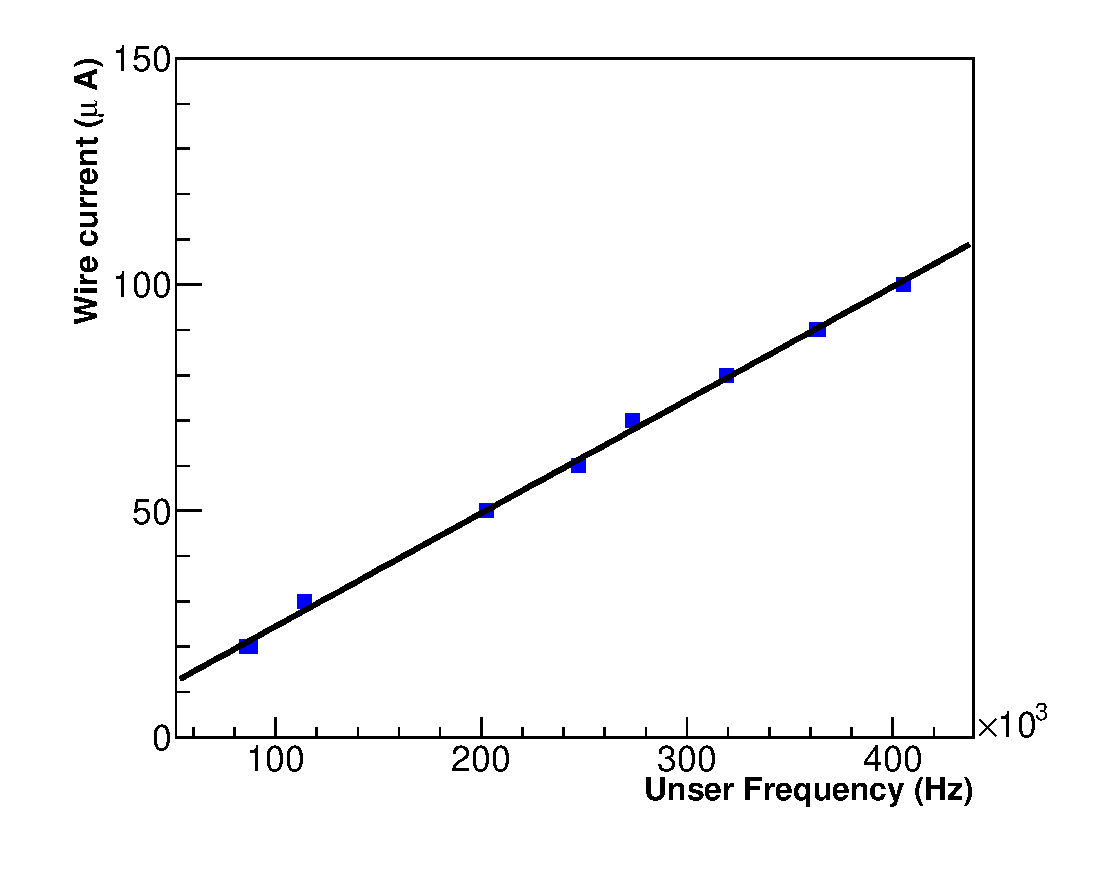
\includegraphics[width=\linewidth]{images/unser_calibration.eps}
    \caption{Wire Unser Calibration.}
    \label{fig:unser_cal}
  \end{minipage}
  \hspace{0.5cm}
  \begin{minipage}[b]{0.5\linewidth}
    \centering
    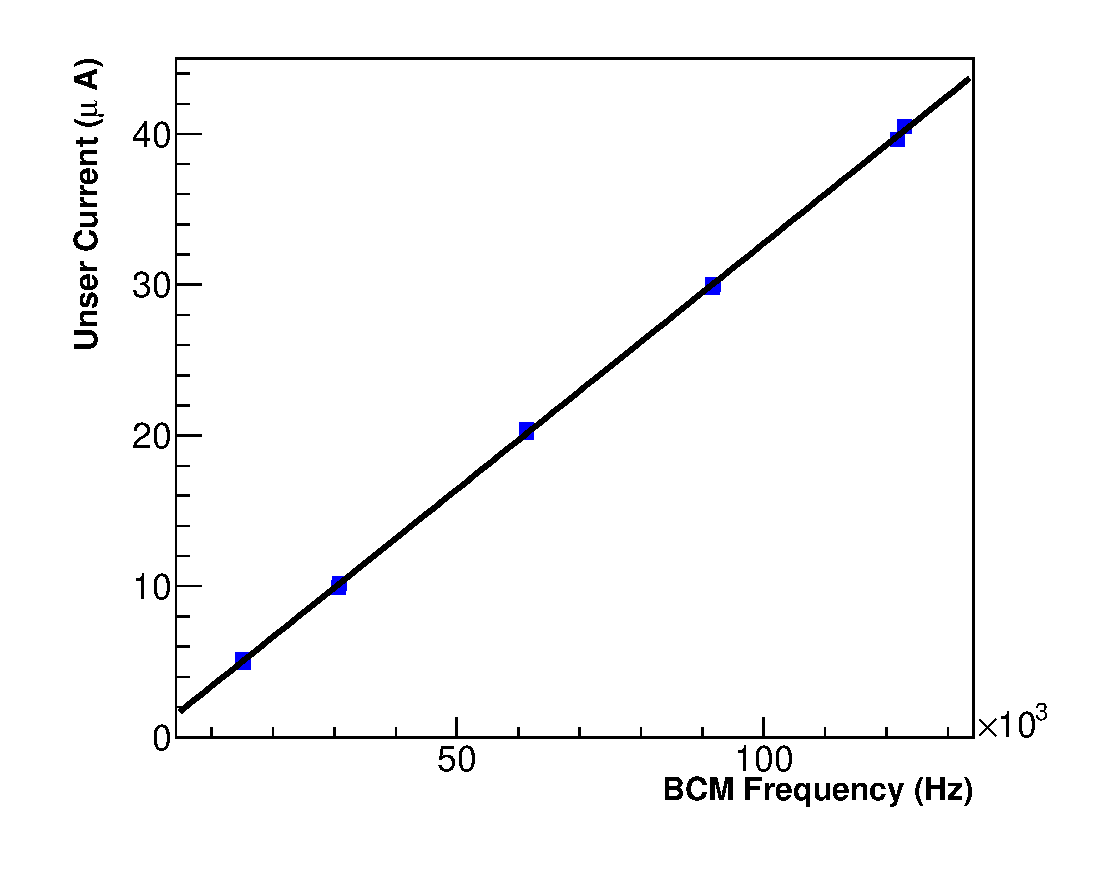
\includegraphics[width=\linewidth]{images/dnew_calibration.eps}
    \caption{BCM calibration.}
    \label{fig:dnew_cal}
  \end{minipage}
\end{figure}

Two stainless steel resonant cavities surround the Unser and are tuned to the frequency of the beam $1.497$ $GHz$ with a quality coefficient $Q \approx 500$.    The cavities are composed of loop antennas located where the magnetic field is maximum. When the beam passes through the output RF signal is proportional to the current \cite{denard}. The BCM response is linear with respect to the current. In the calibration, the accelerator sent a set of currents, which are estimated with the Unser and then used to calculate the linear dependence of the BCM.


Figure \ref{fig:unser_cal} shows the Unser calibration, the gain of the Unser is $0.0002497 \pm 9.648 \times 10^{-7} $ $\mu A/Hz$. The Unser gain remains stable within $0.1$ $\%$ of $4$ $mV/\mu A$. 

The beam current was calculated using the gain of the Unser, this current was used for the calculation of the parameters in the BCM linear response, as it is shown in Figure \ref{fig:dnew_cal}. In general, the beam current can be calculated using the frequency of the BCM using,

\begin{equation}
I = g_{BCM}\cdot f+O
\label{eq:current_calc}
\end{equation}

\noindent where $g_{BCM}$ and $O$ are the fit parameters, which correspond to $0.0003264 \pm 1.406 \times 10^{-6}$ $\mu A/Hz$ and $0.1055 \pm 0.09974$  $\mu A$, respectively. And, $f$ is the given frequency of the BCM.

\section{Method Overview}

The density of the target is known when it is filled, but simulations have shown that the beam current will change the density of the target, and this effect is directly related with the luminosity, and therefore with any cross section measurement \cite{celldes}. It is expected that the density remains stable if the current applied to the gas is constant. The production currents for the experiments were $10$ $\mu A$ and $22.5$ $\mu A$, therefore, the goal is to calculate the density of the targets at those currents.  

In order to measure the density change, the Yield is measured for different currents. After the Yield is calculated, it is normalized with respect to the lowest current Yield, and finally it is assumed when there is not current, the normalized Yield is $1$. The percentage changed in the Normalized Yield corresponds to the density percentage changed in the target. 

\begin{equation}
Y = \frac{PS \cdot N}{ Q \cdot \epsilon \cdot LT }
\label{eq:yield}
\end{equation}

\noindent where $N$ is the number of good electrons, $PS$ is the prescale factor, $Q$ is the charge, $\epsilon $ is the combined efficiencies of detectors, triggers and events selection cuts and $LT$ is the live-time. Each one of these parameters is explained in detail in the following sections.

\subsection{Events Selection}
In order to extract a good electron sample, several cuts were applied to the data. These cuts can be summarized in two groups: Acceptance Cuts, which assure that the events are selected within the spectrometer specifications, and Particle IDentification (PID) Cuts, which focus in the selection of electrons scattered from the gas target. 

\begin{itemize}
\item[i.]Acceptance cuts include the momentum acceptance $dp$ and the angular resolution, the out-of-plane angle $\theta $ and the in-plane angle $\phi $. Specifically, the range used in the study 
are $|dp| < 5 $ ,  $|\theta| < 4  $ and $|\phi| < 3 $.

\item[ii.] The trigger selected required both scintillator planes and the Cherenkov detector (GC) to fire, in order to exclude pions events, and to reduce the dead-time.

\item[iii.]Using the other detectors, it was required only one track on the VDC, a GC signal bigger than $2000$, a total energy in the the Calorimeters greater than $1.7$ $GeV$  and smaller than $2.3$ $GeV$. Furthermore,  $E/P>0.7$ was required, where $E$ and $P$ are the electrons energy and momentum, respectively.
\end{itemize}

\subsection{Efficiencies Estimations } 

The efficiencies incorporated in this study include the detectors and trigger capabilities of measurement, and the cuts effects. Specifically, they can be descibed as, 

\begin{itemize}
\item Only electrons with one track in the VDC were selected. Therefore, the ratio between the total of particles with one track with respect to non plus multiple track corresponds to the VDC total efficiency. 
\item The trigger efficiency was calculated using other trigger type, where only both scintillators were used to record the events. In this sense, the difference between the main trigger and the efficiency trigger is the Cherenkov detector.  The ratio between the events recorded with the main and the efficiency trigger corresponds to the trigger efficiency.
\item The Cherenkov efficiency was calculated by selecting a clean sample of electrons detected in the Calorimeters detectors, and counting the number of events that also were detected in the Cherenkov detector.

\item The Calorimeters efficiency was measured by selecting a clean sample of electrons in the Cherenkov detector and counting the number of electrons that also fired the Calorimeters.

\end{itemize}


\subsection{Live-Time Calculation } 

The live-time is related with the limitation of the speed of DAQ system to process the events into the hard disk. It is dependent on the electronics, computers and trigger rate and is calculated using the ratio between the number of events recorded over the total number of events seen by the trigger. 



\subsection{ Total Charge}

The beam is not completely stable in all the run, it may trip or fluctuate overtime. Therefore, the number of events and the charge is calculated only if the average current is within a window of $\pm 2$ $\mu A$ of the current asked to the accelerator.  The charge is calculated using BCM calibration result integrated over time.


\section{Solid Target Check}

The aim of the analysis is to measure the density change when the beam is on the gas targets using the Yield analysis. In order to test the method, the same analysis is implemented in a solid target, in particular, in the $^{40}Ar$ experiment using a carbon foil, and in the Tritium experiment using an aluminum target. When a solid target is used, the density does not vary and therefore, the Yield should be constant for any given current.

\begin{figure}[htbp]
  \begin{minipage}[b]{0.5\linewidth}
    \centering
    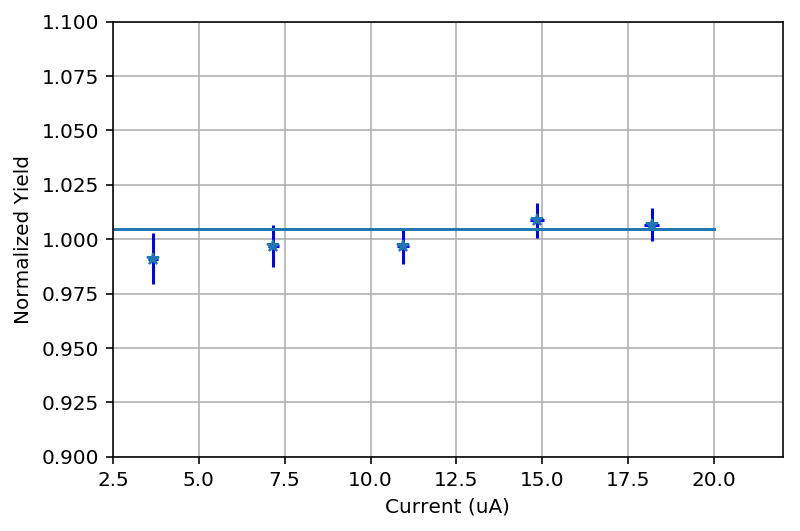
\includegraphics[width=\linewidth]{images/argon_solid.png}
    \caption{$C$ Yield analysis for the $^{40}Ar$ experiment.}
    \label{fig:ar_solid}
  \end{minipage}
  \hspace{0.5cm}
  \begin{minipage}[b]{0.5\linewidth}
    \centering
    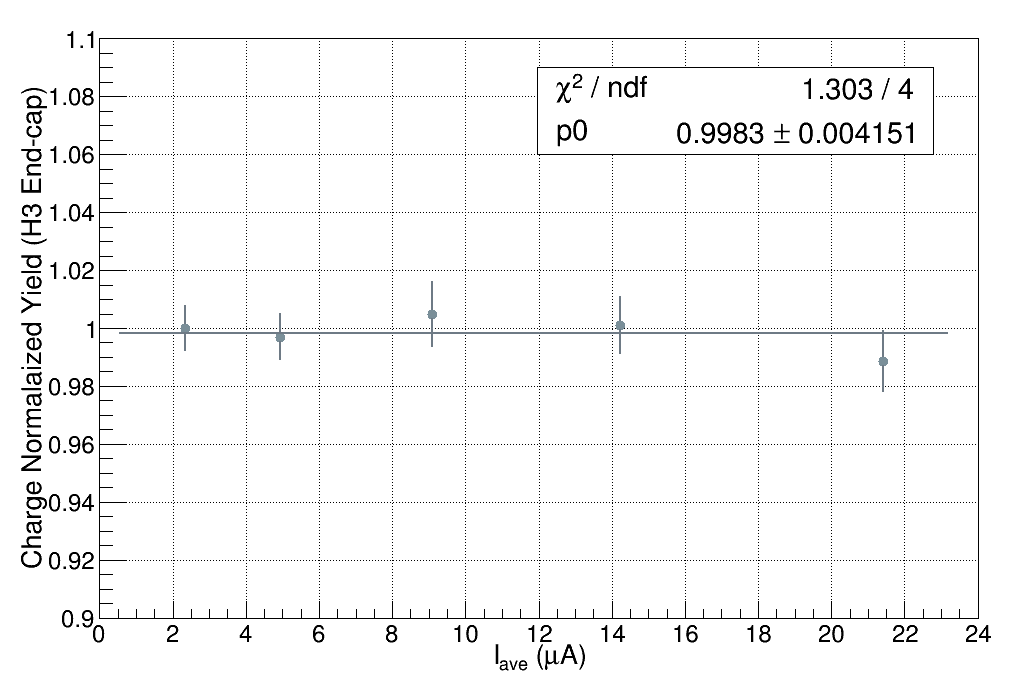
\includegraphics[width=\linewidth]{images/upstream.png}
    \caption{$Al$ Yield analysis for the Tritium experiments. }
    \label{fig:3H_solid}
  \end{minipage}
\end{figure}

Figure \ref{fig:ar_solid} and Figure \ref{fig:3H_solid}, show the Normalized Yield of the solid targets for the $^{40}Ar$ and Tritium set of experiments. For this plots, the Yield was calculated using Equation \ref{eq:yield} for the the different beam currents and it was normalized with respect to the average Yield value. As it can be seen in both figures, the Yield is constant within one percent of the average value. As a result, the plots prove that for a solid target, the Yield is independent on the current since the density of the target remains constant.

\section{Background Contamination}

The aluminum end-caps of the target cell contribute in the Yield calculation of the gas targets. Therefore, dummy cell measurements with aluminum foils of identical properties that the end-caps of the gas targets were taken, in order to remove the background events coming from the aluminum.

In order to check how end-cap background changes with increasing current, a
comparison between the background at low and high current was estimated for
an empty cell (Figure \ref{fig:bk_empty}). Each run was normalized over the total charge yield, and the ratio of the events at high current to low current was estimated. The ratio was found to be 1.006, which indicates that the end-cap background will not increase with increasing current and it is a constant number. Therefore, for the charge normalized yield this value will cancel out. However, when calculating the total charge yield, the background events need to be extracted from cryotarget events.

\begin{figure}[h]
 \centering
 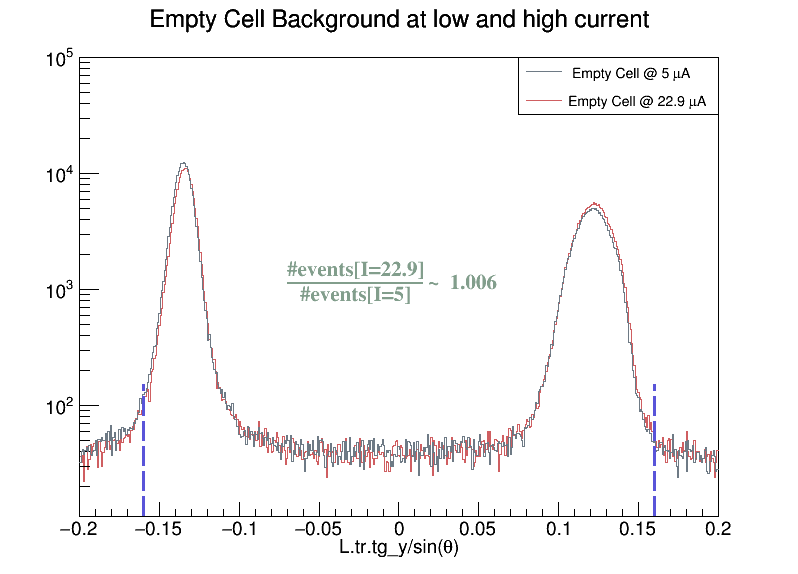
\includegraphics[width=0.6\linewidth]{images/bk_empty.png}
  \caption{Ratio of end-cap background at high current to low current}
  \label{fig:bk_empty}
\end{figure}

 
 
\section{Gas Target Results}


\section{Acknowledgments}
%% \label{}

\bibliographystyle{elsarticle-num} 
\bibliography{references.bib}

\end{document}
\endinput
%%
%% End of file `elsarticle-template-num.tex'.
